\section{1174021 - Muhammad Fahmi}
\subsection{Soal Teori}
\begin{enumerate}

	\item Jelaskan kenapa file teks harus di lakukan tokenizer. dilengkapi dengan ilustrasi atau gambar.
	\hfill\break
	Karena MTokenizer merupakan proses membagi teks yang dapat berupa kalimat, paragraf atau dokumen menjadi kata-kata atau bagian-bagian tertentu dalam kalimat tersebut. Sebagai contoh dari kalimat "Cieee yang copas punya fahmi", kalimat itu menjadi beberapa bagian yaitu "cieee", "yang", "copas", "punya", "fahmi". Yang menjadi acuan yakni tanda baca dan spasi. Untuk ilustrasi, lihat gambar berikut: 

	\begin{figure}[H]
	\centering
		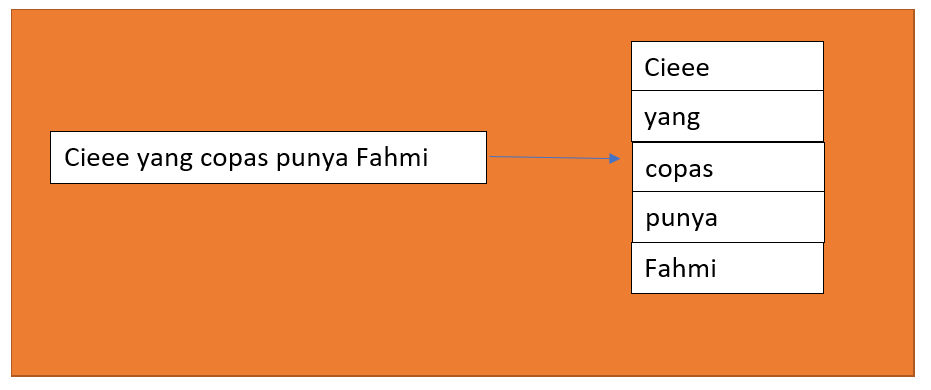
\includegraphics[width=4cm]{figures/1174021/tugas7/materi/teori1.PNG}
		\caption{Teori 1}
	\end{figure}

	\item Jelaskan konsep dasar K Fold Cross Validation pada dataset komentar Youtube pada kode listing 7.1. dilengkapi dengan ilustrasi atau gambar.

	\lstinputlisting[firstline=8, lastline=9]{src/1174021/tugas7/teori.py}

	\hfill\break
	Konsep sederhana dari K Fold Cross Validation ialah Pada code tesebut terdapat kfold yang bertujuan untuk melakukan split data menjadi 5 bagian dari dataset komentar Youtube tersebut. Sehingga dari setiap data yang sudah dibagi tersebut akan menghasilkan presentase dari setiap bagiannya, untuk menghasilkan hasil akhir dengan presentase yang cukup baik. Untuk ilustrasi, lihat gambar berikut: 

	\begin{figure}[H]
	\centering
		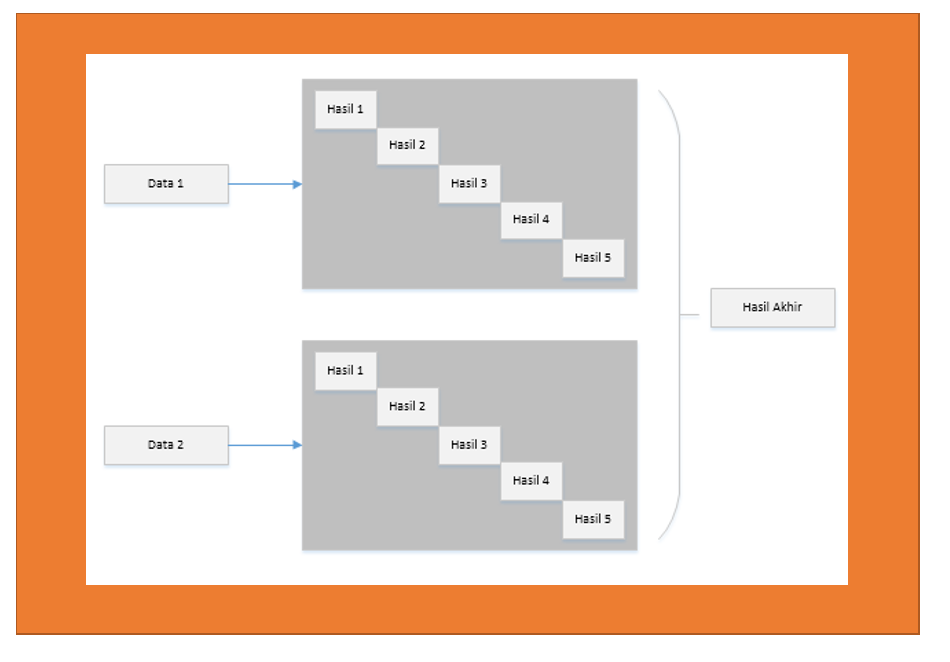
\includegraphics[width=4cm]{figures/1174021/tugas7/materi/teori2.PNG}
		\caption{Teori 2}
	\end{figure}
	
	\item Jelaskan apa maksudnya kode program for train, test in splits.dilengkapi dengan ilustrasi atau gambar.

	\hfill\break
	Untuk penjelasan nya yaitu For train berfungsi untuk membagi data tersebut menjadi data training. Sedangkan test in splits berfungsi untuk menguji apakah dataset tersebut sudah dibagi menjadi beberapa bagian atau masih menumpuk. Untuk ilustrasi, lihat gambar berikut: 

	\begin{figure}[H]
	\centering
		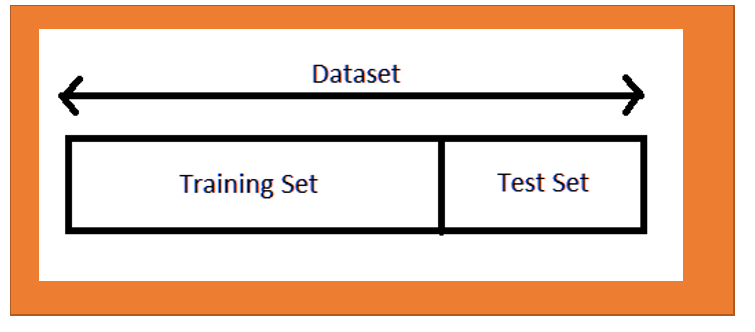
\includegraphics[width=4cm]{figures/1174021/tugas7/materi/teori3.PNG}
		\caption{Teori 3}
	\end{figure}

	\item Jelaskan apa maksudnya kode program train content = d[’CONTENT’].iloc[train idx] dan test content = d[’CONTENT’].iloc[test idx]. dilengkapi dengan ilustrasi atau gambar.

	\hfill\break
	Fungsi dalam kode tersebut berfungsi untuk mengambil data pada kolom atau index CONTENT yang merupakan bagian dari train\_idx dan test\_idx. Contoh sederhananya ketika data telah diubah menjadi data train dan data test maka kita dapat memilihnya untuk ditampilkan pada kolom yang di inginkan. Namun, untuk ilustrasi lihat gambar berikut: 

	\lstinputlisting[firstline=14, lastline=21]{src/1174021/tugas7/teori.py}

	\begin{figure}[H]
	\centering
		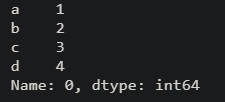
\includegraphics[width=4cm]{figures/1174021/tugas7/materi/teori4.PNG}
		\caption{Teori 4}
	\end{figure}

	\item Jelaskan apa maksud dari fungsi tokenizer = Tokenizer(num words=2000) dan tokenizer.fit on texts(train content), dilengkapi dengan ilustrasi atau gambar.
	\hfill\break
	Fungsi tokenizer ini berfungsi untuk melakukan vektorisasi data kedalam bentuk token sebanyak 2000 kata. Dan selanjutnya akan melakukan fit tokenizer hanya untuk data training saja tidak dengan data testingnya. Untuk ilustrasi lihat gambar berikut: 

	\begin{figure}[H]
	\centering
		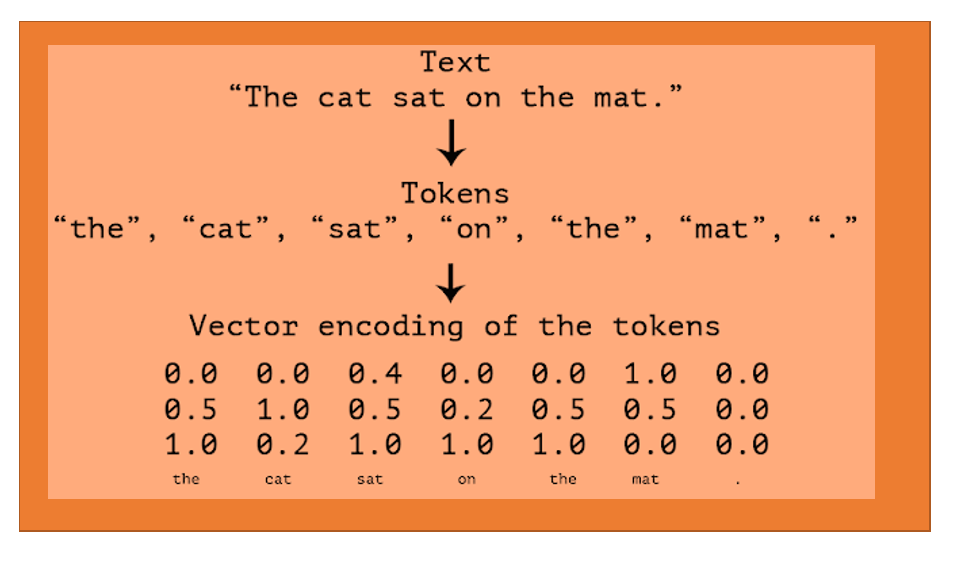
\includegraphics[width=4cm]{figures/1174021/tugas7/materi/teori5.PNG}
		\caption{Teori 5}
	\end{figure}

	\item Jelaskan apa maksud dari fungsi d train inputs = tokenizer.texts to matrix(train content, mode=’tfidf ’) dan d test inputs = tokenizer.texts to matrix(test content, mode=’tfidf ’), dilengkapi dengan ilustrasi kode dan atau gambar.
	\hfill\break
	Maksud dari baris diatas ialah untuk memasukkan text ke sebuah matrix dengan mode tfidf dan menginputkan data testing untuk di terjemahkan ke sebuah matriks. Untuk ilustrasi, lihat gambar berikut: 

	\begin{figure}[H]
	\centering
		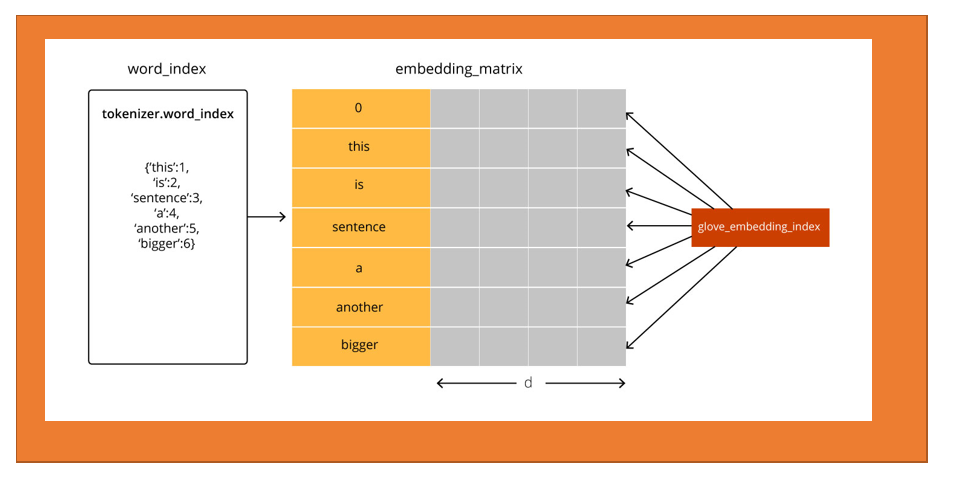
\includegraphics[width=4cm]{figures/1174021/tugas7/materi/teori6.PNG}
		\caption{Teori 6}
	\end{figure}

	\item Jelaskan apa maksud dari fungsi d train inputs = d train inputs/np.amax(np.absolute(d train inputs)) dan d test inputs = d test inputs/np.amax(np.absolute(d test inputs)), dilengkapi dengan ilustrasi atau gambar.
	\hfill\break
	Fungsi np.amax adalah nilai Maksimal. Jika sumbu tidak ada, hasilnya adalah nilai skalar. Jika sumbu diberikan, hasilnya adalah array dimensi a.ndim - 1. Untuk ilustrasi, lihat gambar berikut: 

	\begin{figure}[H]
	\centering
		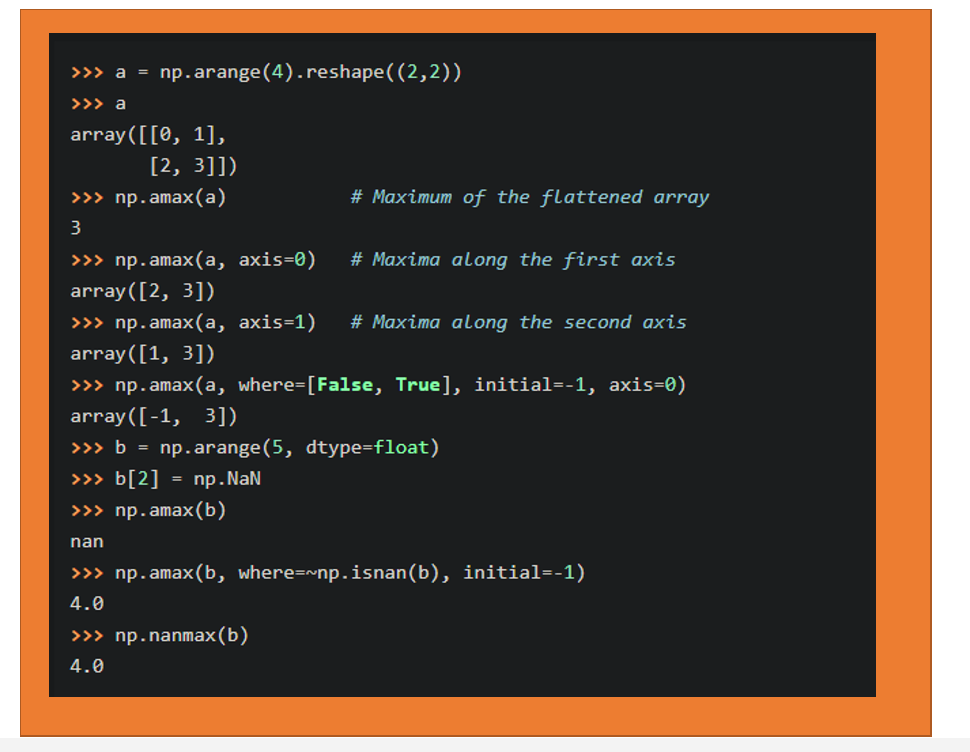
\includegraphics[width=4cm]{figures/1174021/tugas7/materi/teori7.PNG}
		\caption{Teori 7}
	\end{figure}

	\item Jelaskan apa maksud fungsi dari d train outputs = np utils.to categorical(d[’CLASS’].iloc[train idx]) dan d test outputs = np utils.to categorical(d[’CLASS’].iloc[test idx]) dalam kode program, dilengkapi dengan ilustrasi atau gambar.
	\hfill\break
	Fungsi dari baris kode tersebut ialah membuat train outputs dengan kategori dari class lalu dengan ketentuan iloc train idx. Kemudian membuat keluaran sebagai output. Untuk ilustrasi, lihat gambar berikut: 

	\begin{figure}[H]
	\centering
		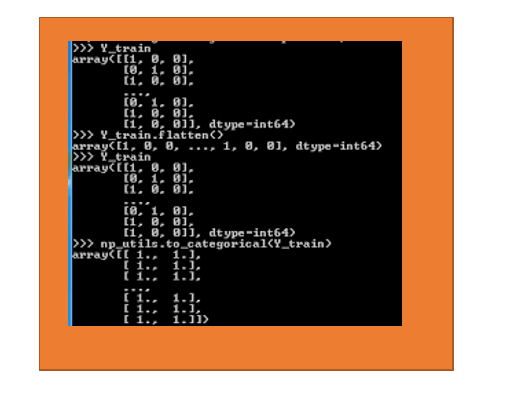
\includegraphics[width=4cm]{figures/1174021/tugas7/materi/teori8.PNG}
		\caption{Teori 8}
	\end{figure}

	\item Jelaskan apa maksud dari fungsi di listing 7.2. Gambarkan ilustrasi Neural Network nya dari model kode tersebut.
	\hfill\break

	\lstinputlisting[firstline=27, lastline=32]{src/1174021/tugas7/teori.py}

	Fungsi dari baris kode tersebut ialah model perlu mengetahui bentuk input apa yang harus diharapkan. Untuk alasan ini, lapisan pertama dalam model Sequential (dan hanya yang pertama, karena lapisan berikut dapat melakukan inferensi bentuk otomatis) perlu menerima informasi tentang bentuk inputnya.

	\begin{figure}[H]
	\centering
		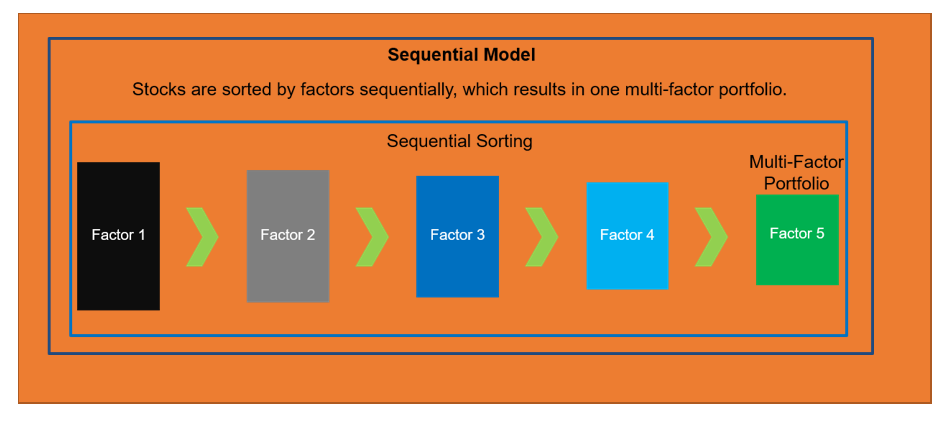
\includegraphics[width=4cm]{figures/1174021/tugas7/materi/teori9.PNG}
		\caption{Teori 9}
	\end{figure}

	\item Jelaskan apa maksud dari fungsi di listing 7.3 dengan parameter tersebut.
	\hfill\break

	\lstinputlisting[firstline=35, lastline=36]{src/1174021/tugas7/teori.py}

	Fungsi dari baris kode tersebut ialah bisa meneruskan nama fungsi loss yang ada, atau melewati fungsi simbolis TensorFlow yang mengembalikan skalar untuk setiap titik data dan mengambil dua argumen y\_true: True label. dan  y\_pred: Prediksi. Tujuan yang dioptimalkan sebenarnya adalah rata-rata dari array output di semua titik data.

	\begin{figure}[H]
	\centering
		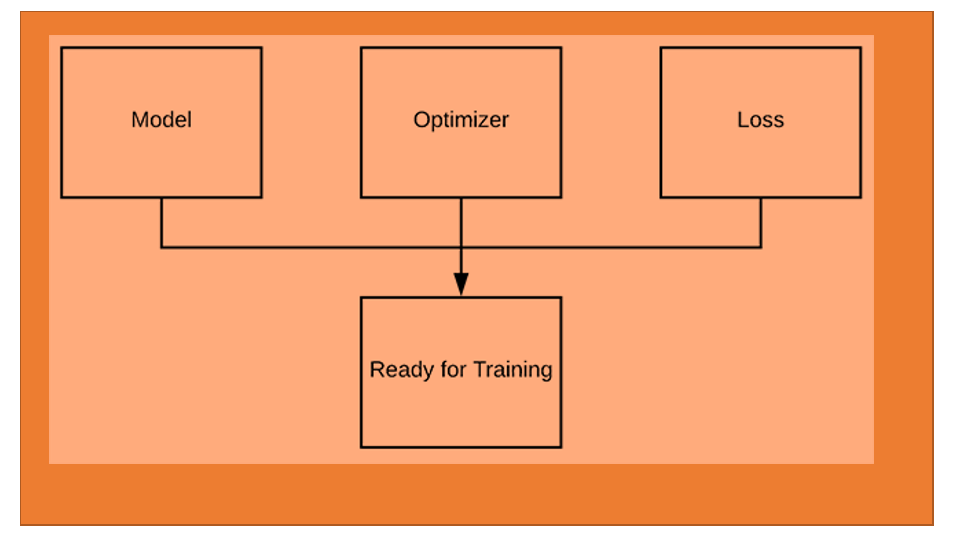
\includegraphics[width=4cm]{figures/1174021/tugas7/materi/teori10.PNG}
		\caption{Teori 10}
	\end{figure}

	\item Jelaskan apa itu Deep Learning.
	\hfill\break

	Deep Learning adalah salah satu cabang dari ilmu machine learning yang terdiri dari algoritma pemodelan abstraksi tingkat tinggi pada data menggunakan sekumpulan fungsi transformasi non-linear yang ditata berlapis-lapis dan mendalam. Teknik dan algoritma dalam machine learning dapat digunakan baik untuk supervised learning dan unsupervised learning.

	\item Jelaskan apa itu Deep Neural Network, dan apa bedanya dengan Deep Learning.
	\hfill\break

	DNN adalah salah satu algoritma berbasis jaringan saraf tiruan yang memiliki dari 1 lapisan saraf tersembunyi yang dapat digunakan untuk pengambilan keputun. Perbedaannya dengan deep learning, yakni: DNN dapat menentukan dan mencerna karakteristik tertentu di suatu rangkaian data, kapabilitas lebih kompleks untuk mempelajari, mencerna, dan mengklasifikasikan data, serta dibagi ke dalam berbagai lapisan dengan fungsi yang berbeda-beda.

	\item Jelaskan dengan ilustrasi gambar buatan sendiri(langkah per langkah) bagaimana perhitungan algoritma konvolusi dengan ukuran stride (NPM mod3+1) x (NPM mod3+1) yang terdapat max pooling.
	\hfill\break

	1174021 mod3+1 x 1174021 mod3+1 = 2 x 2, adapun ilustrasi gambar nya sebagai berikut : 

	\begin{figure}[H]
	\centering
		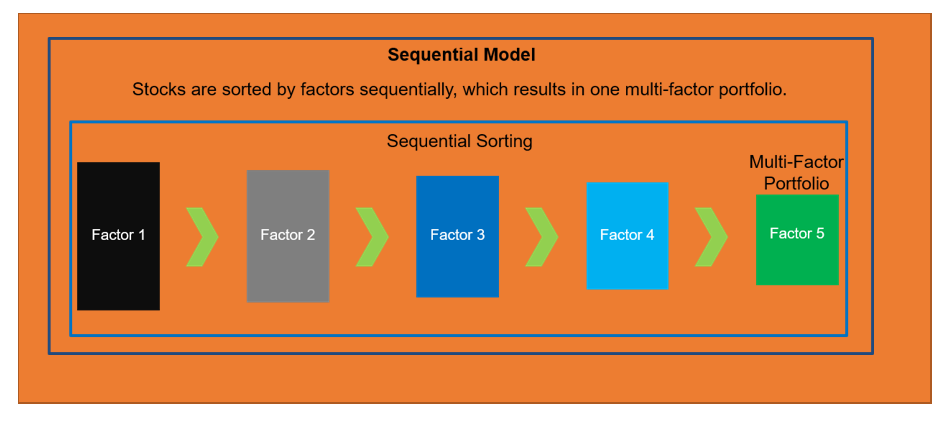
\includegraphics[width=4cm]{figures/1174021/tugas7/materi/teori9.PNG}
		\caption{Teori 9}
	\end{figure}
\end{enumerate}

\subsection{Praktek Program}
\begin{enumerate}
	\item Soal 1
	\hfill\break
	\lstinputlisting[firstline=8, lastline=14]{src/1174021/tugas7/tugas7.py}
	Kode di atas menjelaskan tentang library yang akan di pakai yaitu import file csv, lalu load module pil image dan juga import library keras, hasilnya adalah sebagai berikut:
	\begin{figure}[H]
	\centering
		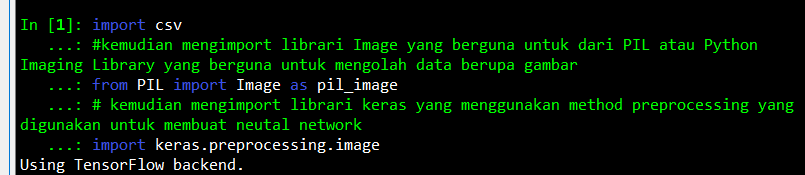
\includegraphics[width=4cm]{figures/1174021/tugas7/materi/hasil1.PNG}
		\caption{Hasil Soal 1.}
	\end{figure}

	\item Soal 2
	\hfill\break
	\lstinputlisting[firstline=16, lastline=42]{src/1174021/tugas7/tugas7.py}
	Kode di atas akan menampilkan hasil dari proses load dataset dari HASYv2 sebagai file csv, membuat variabel i dengan parameter 0, lalu perintah perulangan if dengan i>0, variabel img dengan nilai 255.0, imgs.append yaitu  proses melampirkan atau menggabungkan data dengan file. Berikut adalah hasil setelah saya lakukan running dan pembacaan file audio :
	\begin{figure}[H]
	\centering
		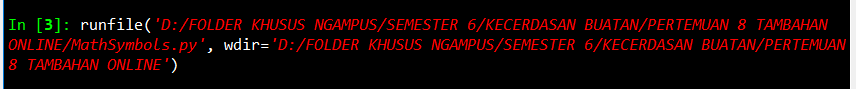
\includegraphics[width=4cm]{figures/1174021/tugas7/materi/hasil2.PNG}
		\caption{Hasil Soal 2.}
	\end{figure}

	\item Soal 3
	\hfill\break
	\lstinputlisting[firstline=44, lastline=54]{src/1174021/tugas7/tugas7.py}
	Perintah import random yaitu sebagai library untuk menghasilkan nilai acak, disini kita membuat data menjadi 2 bagian yaitu 80\% sebagai training dan 20\% sebagai data testing. Hasilnya adalah sebagai berikut :
	\begin{figure}[H]
	\centering
		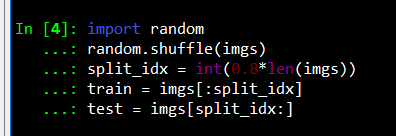
\includegraphics[width=4cm]{figures/1174021/tugas7/materi/hasil3.PNG}
		\caption{Hasil Soal 3.}
	\end{figure}

	\item Soal 4
	\hfill\break
	\lstinputlisting[firstline=56, lastline=66]{src/1174021/tugas7/tugas7.py}
	Kode di atas dapat digunakan untuk melakukan fungsi yang sebelumnya telah kita lakukan yaitu dengan membuat variabel baru untuk menampung data train input dan test input lalu keluaran nya sebagai output, . Hasilnya adalah sebagai berikut :
	\begin{figure}[H]
	\centering
		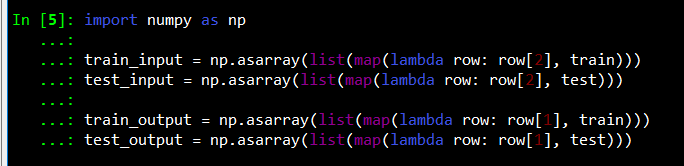
\includegraphics[width=4cm]{figures/1174021/tugas7/materi/hasil4.PNG}
		\caption{Hasil Soal 4.}
	\end{figure}

	\item Soal 5
	\hfill\break
	\lstinputlisting[firstline=68, lastline=72]{src/1174021/tugas7/tugas7.py}
	Kode diatas untuk melakukan import library yang berfungsi sebagai label encoder dan one hot encoder. Hasilnya adalah sebagai berikut :
	\begin{figure}[H]
	\centering
		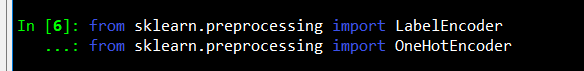
\includegraphics[width=4cm]{figures/1174021/tugas7/materi/hasil5.PNG}
		\caption{Hasil Soal 5.}
	\end{figure}

	\item Soal 6
	\hfill\break
	\lstinputlisting[firstline=74, lastline=79]{src/1174021/tugas7/tugas7.py}
	Kode diatas berfungsi untuk melakukan convert class names ke one-hot encoding. Hasilnya adalah sebagai berikut :
	\begin{figure}[H]
	\centering
		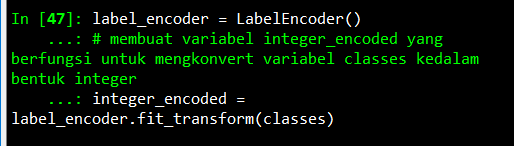
\includegraphics[width=4cm]{figures/1174021/tugas7/materi/hasil6.PNG}
		\caption{Hasil Soal 6.}
	\end{figure}

	\item Soal 7
	\hfill\break
	\lstinputlisting[firstline=81, lastline=87]{src/1174021/tugas7/tugas7.py}
	Kode di atas befungsi untuk melakukan convert integers ke fungsi one hot encoding. Hasilnya adalah sebagai berikut :
	\begin{figure}[H]
	\centering
		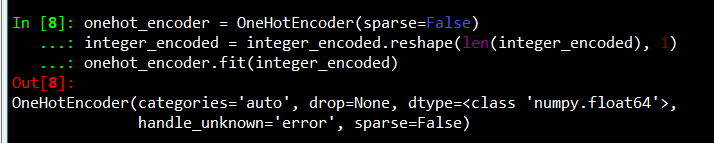
\includegraphics[width=4cm]{figures/1174021/tugas7/materi/hasil7.PNG}
		\caption{Hasil Soal 7.}
	\end{figure}

	\item Soal 8
	\hfill\break
	\lstinputlisting[firstline=89, lastline=101]{src/1174021/tugas7/tugas7.py}
	Kode di atas befungsi untuk melakukan convert train dan test output ke fungsi one hot encoding. Hasilnya adalah sebagai berikut :
	\begin{figure}[H]
	\centering
		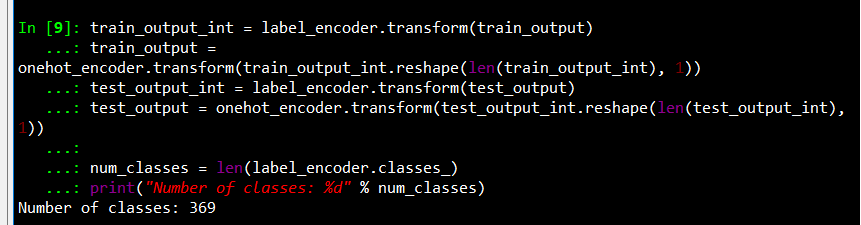
\includegraphics[width=4cm]{figures/1174021/tugas7/materi/hasil8.PNG}
		\caption{Hasil Soal 8.}
	\end{figure}

	\item Soal 9
	\hfill\break
	\lstinputlisting[firstline=103, lastline=109]{src/1174021/tugas7/tugas7.py}
	Kode di atas befungsi untuk melakukan import sequential dari library keras. Hasilnya adalah sebagai berikut : 
	\begin{figure}[H]
	\centering
		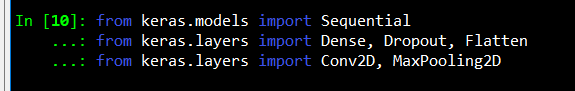
\includegraphics[width=4cm]{figures/1174021/tugas7/materi/hasil9.PNG}
		\caption{Hasil Soal 9.}
	\end{figure}

	\item Soal 10
	\hfill\break
	\lstinputlisting[firstline=111, lastline=135]{src/1174021/tugas7/tugas7.py}
	Kode di atas befungsi untuk melihat detail desain pada jaringan model yang telah di defenisikan. Hasilnya adalah sebagai berikut : 
	\begin{figure}[H]
	\centering
		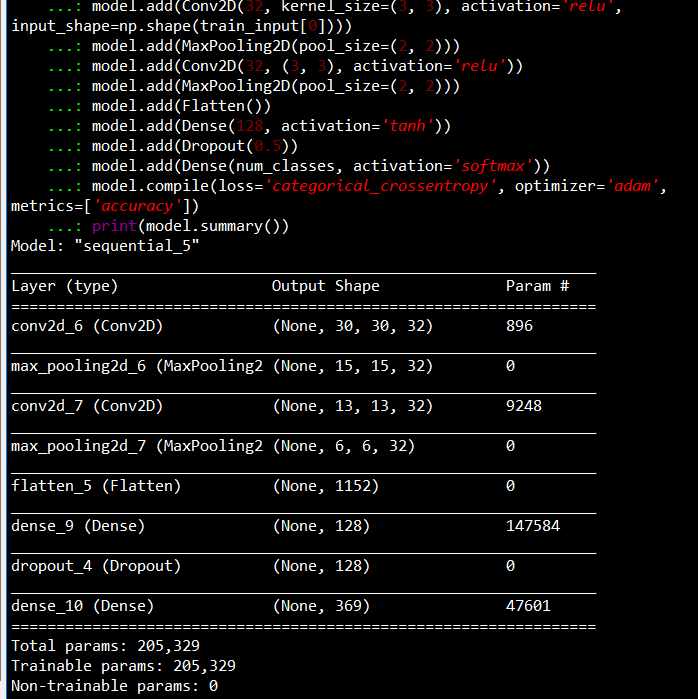
\includegraphics[width=4cm]{figures/1174021/tugas7/materi/hasil10.PNG}
		\caption{Hasil Soal 10.}
	\end{figure}

	\item Soal 11
	\hfill\break
	\lstinputlisting[firstline=137, lastline=142]{src/1174021/tugas7/tugas7.py}
	Kode di atas befungsi untuk melakukan load callbacks pada library keras. Hasilnya adalah sebagai berikut : 
	\begin{figure}[H]
	\centering
		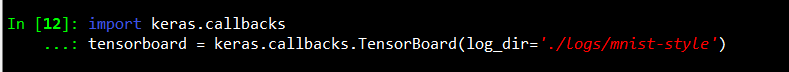
\includegraphics[width=4cm]{figures/1174021/tugas7/materi/hasil11.PNG}
		\caption{Hasil Soal 11.}
	\end{figure}

	\item Soal 12
	\hfill\break
	\lstinputlisting[firstline=143, lastline=155]{src/1174021/tugas7/tugas7.py}
	Kode di atas befungsi untuk melakukan load epoch yang akan di training dan diberikan hasil selama 10 kali epoch. Hasilnya adalah sebagai berikut :  
	\begin{figure}[H]
	\centering
		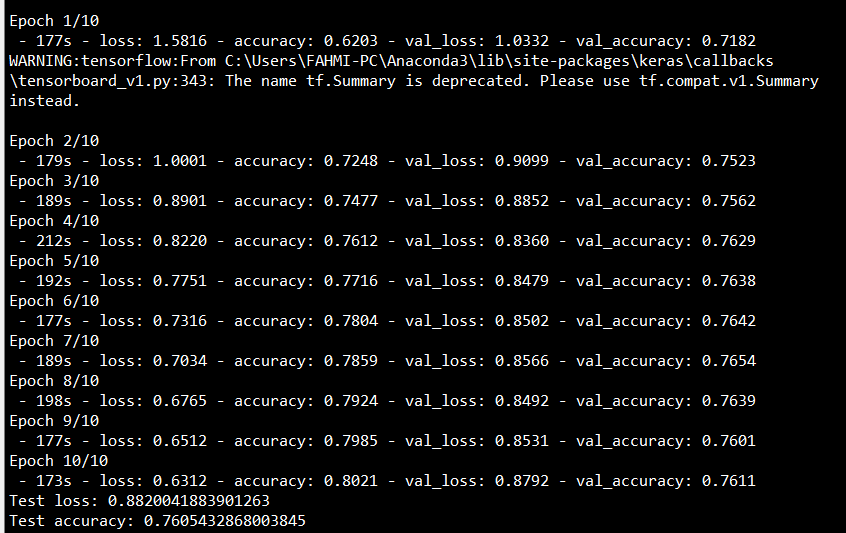
\includegraphics[width=4cm]{figures/1174021/tugas7/materi/hasil12.PNG}
		\caption{Hasil Soal 12.}
	\end{figure}

	\item Soal 13
	\hfill\break
	\lstinputlisting[firstline=157, lastline=212]{src/1174021/tugas7/tugas7.py}
	Kode di atas befungsi untuk melakukan konfigurasi model dengan parameter yang ditentukan dan mencoba mencari data yang terbaik. Hasilnya adalah sebagai berikut :  
	\begin{figure}[H]
	\centering
		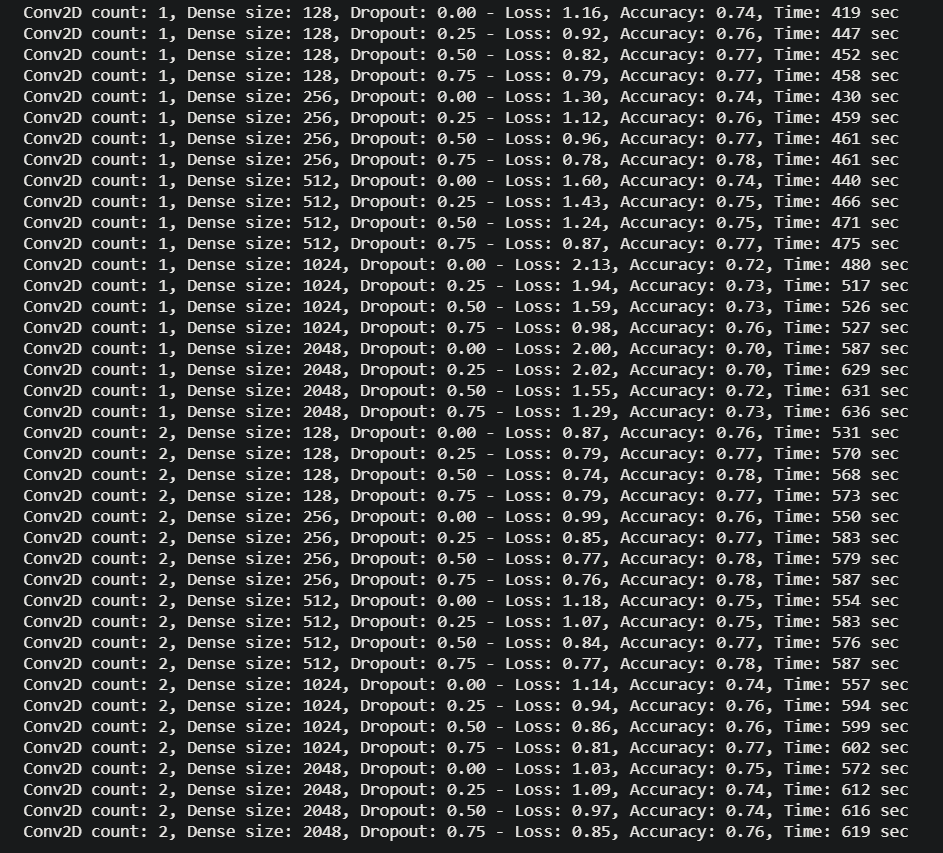
\includegraphics[width=4cm]{figures/1174021/tugas7/materi/hasil13.PNG}
		\caption{Hasil Soal 13.}
	\end{figure}

	\item Soal 14
	\hfill\break
	\lstinputlisting[firstline=215, lastline=237]{src/1174021/tugas7/tugas7.py}
	Kode di atas befungsi untuk membuat data training kembali dengan model yang sudah di tentukan dan mencari yang terbaik dari hasil training tersebut. Hasilnya adalah sebagai berikut :  
	\begin{figure}[H]
	\centering
		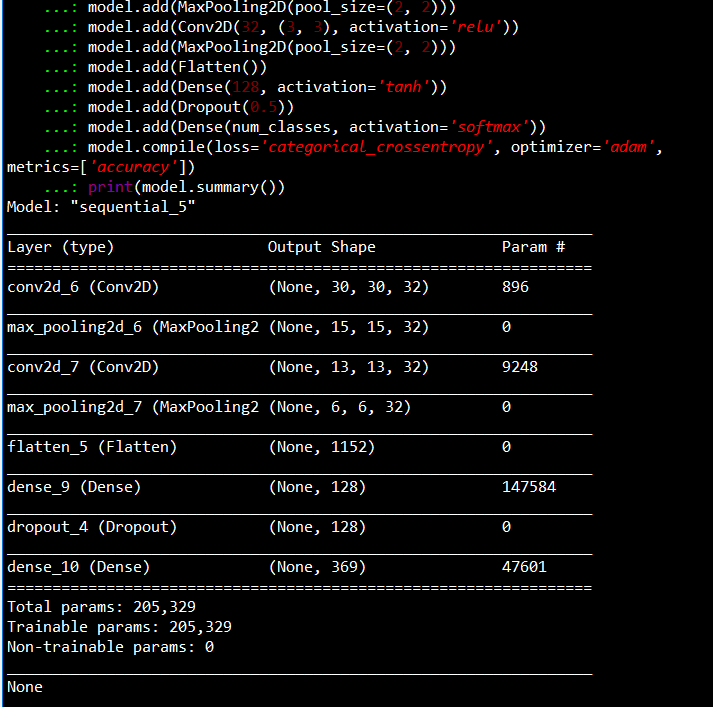
\includegraphics[width=4cm]{figures/1174021/tugas7/materi/hasil14.PNG}
		\caption{Hasil Soal 14.}
	\end{figure}

	\item Soal 15
	\hfill\break
	\lstinputlisting[firstline=238, lastline=244]{src/1174021/tugas7/tugas7.py}
	Kode di atas befungsi untuk melakukan join terhadap data train dan test dengan seluruh konfigurasi yang telah di tentukan sebelumnya. Hasilnya adalah sebagai berikut :  
	\begin{figure}[H]
	\centering
		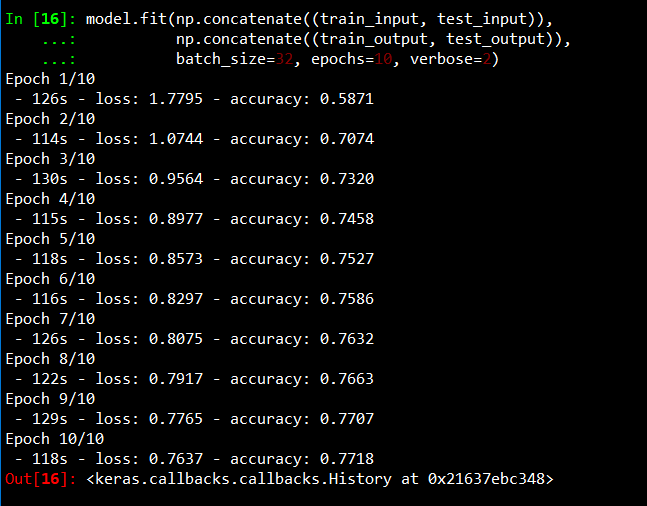
\includegraphics[width=4cm]{figures/1174021/tugas7/materi/hasil15.PNG}
		\caption{Hasil Soal 15.}
	\end{figure}

	\item Soal 16
	\hfill\break
	\lstinputlisting[firstline=246, lastline=248]{src/1174021/tugas7/tugas7.py}
	Kode di atas befungsi untuk melakukan save pada model yang akan disimpan sebagai mathsymbols.model. Hasilnya adalah sebagai berikut :  
	\begin{figure}[H]
	\centering
		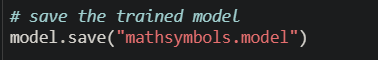
\includegraphics[width=4cm]{figures/1174021/tugas7/materi/hasil16.PNG}
		\caption{Hasil Soal 16.}
	\end{figure}

	\item Soal 17
	\hfill\break
	\lstinputlisting[firstline=250, lastline=252]{src/1174021/tugas7/tugas7.py}
	Kode di atas befungsi untuk melakukan save pada model yang akan disimpan sebagai classes.npy dengan reverse ke fungsi one hot encoding. Hasilnya adalah sebagai berikut :  
	\begin{figure}[H]
	\centering
		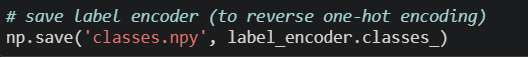
\includegraphics[width=4cm]{figures/1174021/tugas7/materi/hasil17.PNG}
		\caption{Hasil Soal 17.}
	\end{figure}

	\item Soal 18
	\hfill\break
	\lstinputlisting[firstline=255, lastline=262]{src/1174021/tugas7/tugas7.py}
	Kode di atas befungsi untuk melakukan load data yang sudah di train dan juga memprediksikan hasil. Hasilnya adalah sebagai berikut :  
	\begin{figure}[H]
	\centering
		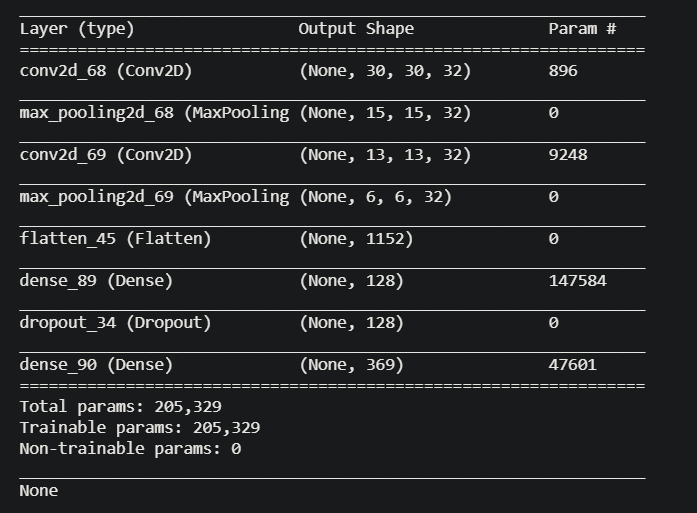
\includegraphics[width=4cm]{figures/1174021/tugas7/materi/hasil18.PNG}
		\caption{Hasil Soal 18.}
	\end{figure}

	\item Soal 19
	\hfill\break
	\lstinputlisting[firstline=264, lastline=284]{src/1174021/tugas7/tugas7.py}
	Kode di atas befungsi untuk melakukan restore terhadap nama class pada fungsi integer encoder, dengan membuat fungsi predict. Hasilnya adalah sebagai berikut :  
	\begin{figure}[H]
	\centering
		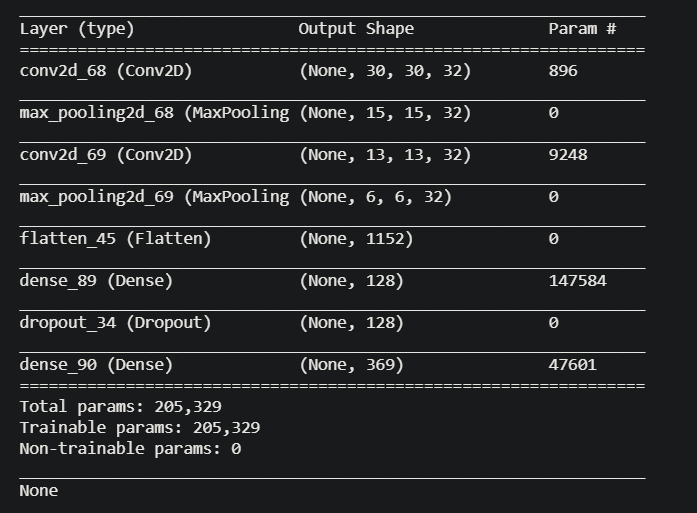
\includegraphics[width=4cm]{figures/1174021/tugas7/materi/hasil19.PNG}
		\caption{Hasil Soal 19.}
	\end{figure}

	\item Soal 20
	\hfill\break
	\lstinputlisting[firstline=286, lastline=292]{src/1174021/tugas7/tugas7.py}
	Kode di atas befungsi untuk menunjukkan hasil akhir prediski. Hasilnya adalah sebagai berikut :  
	\begin{figure}[H]
	\centering
		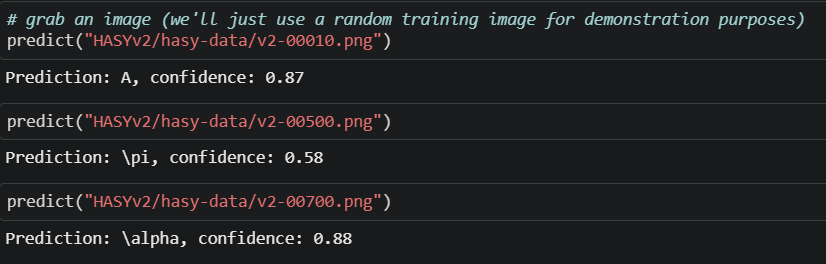
\includegraphics[width=4cm]{figures/1174021/tugas7/materi/hasil20.PNG}
		\caption{Hasil Soal 20.}
	\end{figure}
\end{enumerate}

\subsection{Penanganan Error}
\begin{enumerate}
	\item KeyboardInterrupt
	\begin{figure}[H]
		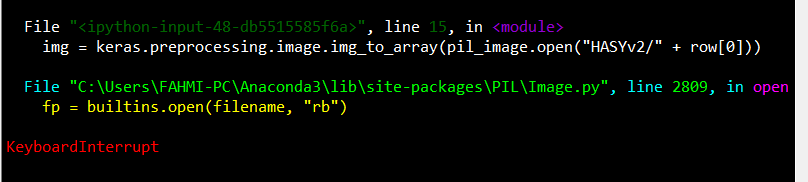
\includegraphics[width=4cm]{figures/1174021/tugas7/error/1.PNG}
		\centering
		\caption{KeyboardInterrupt}
	\end{figure}

	\item Cara Penanganan Error
	\begin{itemize}
		\item KeyboardInterrupt
		\hfill\break
		Error tersebut karena disebabkan oleh human typo yang melakukan klik pada keyboard saat running.
	\end{itemize}
\end{enumerate}

\subsection{Bukti Tidak Plagiat}
\begin{figure}[H]
\centering
	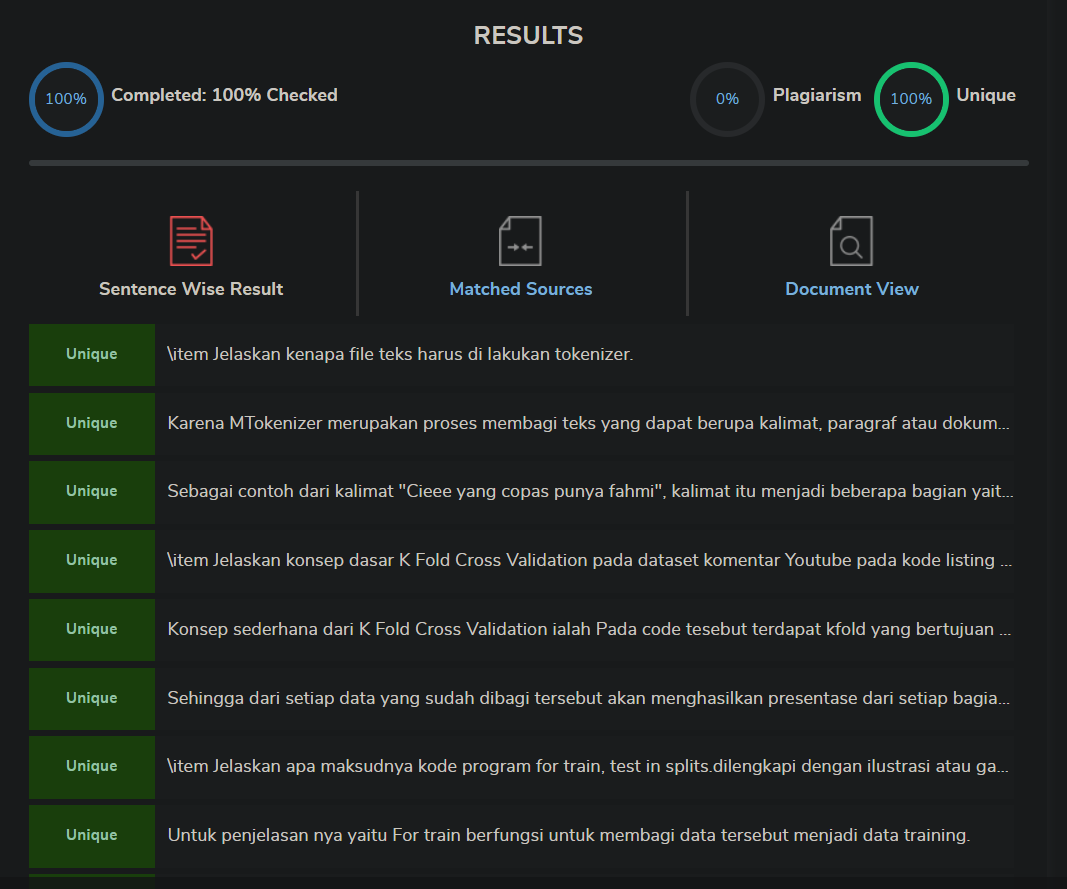
\includegraphics[width=4cm]{figures/1174021/tugas7/buktiplagiat/1.PNG}
	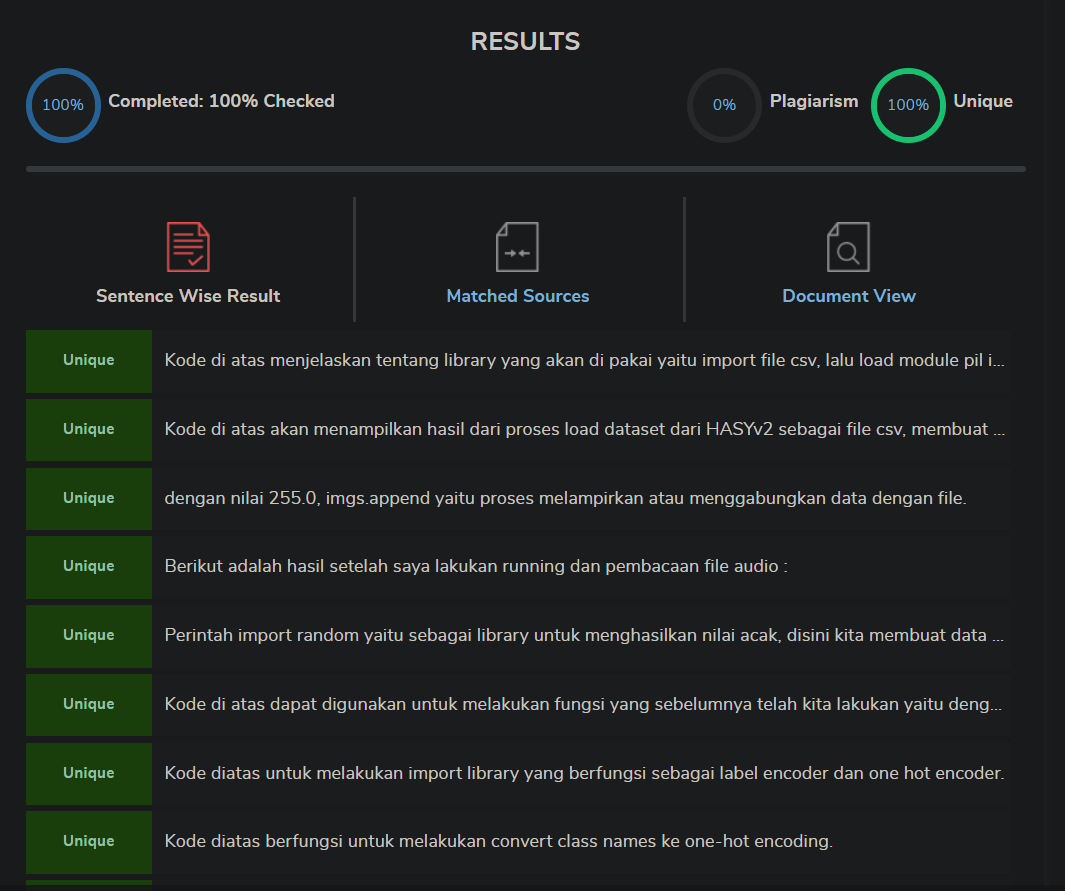
\includegraphics[width=4cm]{figures/1174021/tugas7/buktiplagiat/2.PNG}
	\caption{Bukti Tidak Melakukan Plagiat Chapter 7}
\end{figure}

